\newpage
\section{Auswertung}
\label{sec:Auswertung}
In diesem Abschnitt werden die aufgenommenen Messdaten in Grafiken sowie Tabellen dargestellt und ausgewertet. Grafiken sowie dazugehörige Rechnungen sind mit Python \cite{python} erstellt bzw. berechnet worden.

\subsection{Messung des Magnetfeldes}
\label{sec:magFeld}
Als erstes wird das Magnetfeld am Ort der Probe bestimmt, dazu werden die Messdaten aus Tabelle \ref{tab:magFeld} in Abbildung \ref{abb:magFeld} visualisiert. Dafür wird die Magnetfeldstärke gegen den Ort aufgetragen.
Der maximale Wert $B_\mathrm{max}$ mit dem die weiteren Rechnungen durchgeführt werden ist gegeben durch:
\begin{equation}
  B_\mathrm{max}=\SI{433}{\milli\tesla}
\end{equation}
Dieser legt damit das Magnetfeld am Ort $Z$ der Probe fest.
\begin{figure}[h!]
  \centering
  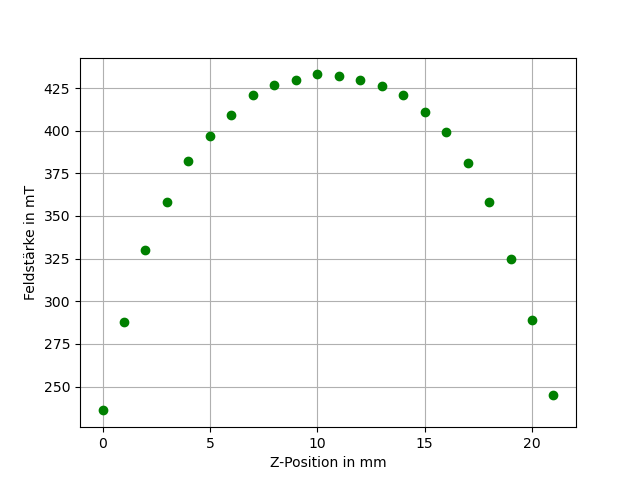
\includegraphics[scale=0.7]{fig/bfeld.png}
  \caption{Zusammenhang zwischen Magnetfeldstärke und Ort im Magnetfeld.}
  \label{abb:magFeld}
\end{figure}
\FloatBarrier

\begin{table}[h!]
  \centering
  \caption{Messdaten der Messung mit der Hallsonde.}
  \label{tab:magFeld}
  \begin{tabular}{c | c}
    \toprule
    Position in $\SI{}{\milli\meter}$ & Magnetfeldstärke in $\SI{}{\milli\tesla}$ \\
    \midrule
    0.0 & 236.0 \\
    1.0 & 288.0 \\
    2.0 & 330.0 \\
    3.0 & 358.0 \\
    4.0 & 382.0 \\
    5.0 & 397.0 \\
    6.0 & 409.0 \\
    7.0 & 421.0 \\
    8.0 & 427.0 \\
    9.0 & 430.0 \\
    10.0 & 433.0 \\
    11.0 & 432.0 \\
    12.0 & 430.0 \\
    13.0 & 426.0 \\
    14.0 & 421.0 \\
    15.0 & 411.0 \\
    16.0 & 399.0 \\
    17.0 & 381.0 \\
    18.0 & 358.0 \\
    19.0 & 325.0 \\
    20.0 & 289.0 \\
    21.0 & 245.0 \\
    \bottomrule
  \end{tabular}
\end{table}
\FloatBarrier
\newpage
\subsection{Messung mit undotiertem Galliumarsenid}
\label{sec:undotiert}
In diesem Auswertungsabschnitt wird die undotierte Galliumarsenid-Probe betrachtet.
Mit der Dicke der Probe $L_\mathrm{undotiert}=\SI{5.11}{\milli\meter}$ und den gemessenen Werten wird ein normierter Wert der Faradayrotation bestimmt. Dazu wird zunächst die Formel (\ref{eqn:rotawinkel}) benutzt um den Differenzwinkel $\vartheta$ zu bestimmen, anschließend
wird dieser Wert in [$\SI{}{\radian\per\milli\meter}$] umgerechnet. Mit Hilfe von Gleichung (\ref{eqn:umrechnung}) wird der normierte Wert $\vartheta_\mathrm{norm,undotiert}$ erhalten. Die Formel für die Umrechnung lautet:
\begin{equation}
  \label{eqn:umrechnung}
  \vartheta_\mathrm{norm}=\dfrac{2\pi}{360}\dfrac{\vartheta}{L_\mathrm{undotiert}}
\end{equation}
In der Tabelle \ref{tab:undot} sind die Messdaten für die verschiedenen Wellenlängen $\lambda$ sowie den dazugehörigen Winkeln $\vartheta_\mathrm{+B}$ und $\vartheta_\mathrm{-B}$, als auch den normierten Rotationswinkel $\vartheta_\mathrm{norm,undotiert}$ zu finden.
In Abbildung \ref{abb:undot} sind die normierten Rotationswinkel $\vartheta_\mathrm{norm,undotiert}$ gegen die Quadrate der Wellenlängen $\lambda^2$ aufgetragen.
\begin{table}
  \centering
  \caption{Messdaten der undotierten Galliumarsenid-Probe und normierte Rotationswinkel in $\SI{}{\radian\per\milli\meter}$.}
  \label{tab:undot}
  \begin{tabular}{c | c | c | c}
    \toprule
    $\lambda$/$\SI{}{\micro\meter}$ & $\vartheta_\mathrm{+B}$/$\SI{}{\degree}$ & $\vartheta_\mathrm{-B}$/$\SI{}{\degree}$& $\vartheta_{\mathrm{norm,undotiert}}$/$\SI{}{\radian\per\milli\meter}$ \\
    \midrule
    1.060 & 276.65 & 253.00 & 0.040 \\
    1.290 & 273.00 & 256.33 & 0.028 \\
    1.450 & 273.00 & 260.50 & 0.021 \\
    1.720 & 270.00 & 262.17 & 0.013 \\
    1.960 & 264.03 & 257.45 & 0.011 \\
    2.156 & 262.00 & 257.08 & 0.008 \\
    2.340 & 236.50 & 231.15 & 0.009 \\
    2.510 & 215.08 & 211.67 & 0.006 \\
    2.650 & 161.41 & 156.15 & 0.009 \\
    \bottomrule
  \end{tabular}
\end{table}
\FloatBarrier

\begin{figure}
  \centering
  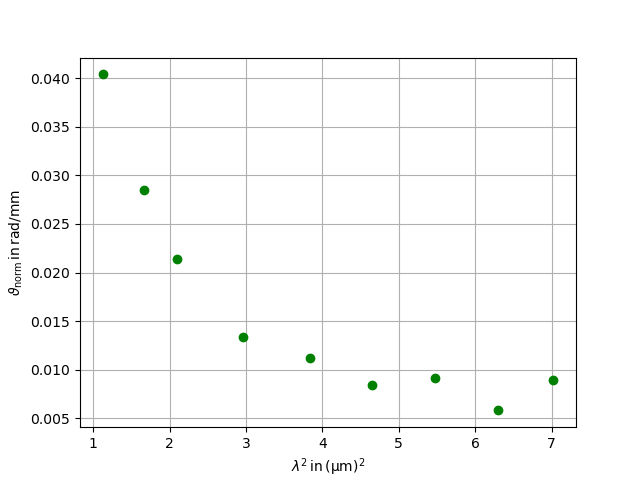
\includegraphics[scale=0.7]{fig/undotiert.png}
  \caption{Grafische Darstellung der Messdaten der undotierten Probe.}
  \label{abb:undot}
\end{figure}
\FloatBarrier

\subsection{Messung mit dotierten Galliumarsenid-Proben}
\label{sec:dot}
In dieser Messung werden nun die dotierten Galliumarsenid-Proben verwendet.
Die zu untersuchenden Proben haben jeweils die Dicken $L_{\mathrm{leicht}}=\SI{1.296}{\milli\meter}$ bzw. $L_{\mathrm{hoch}}=\SI{1.36}{\milli\meter}$ und eine Donatorenkonzentration von $N_{\mathrm{leicht}}=\SI{1.2 e18}{\per\centi\cubic\meter}$ bzw. $N_{\mathrm{hoch}}=\SI{2.8 e18}{\per\centi\cubic\meter}$.
In den Tabellen \ref{tab:tief} und \ref{tab:hoch} sind die erhaltenen Messdaten aufgelistet.
Als erstes wird wieder die Differenz mit Gleichung (\ref{eqn:rotawinkel}) errechnet, daraus werden dann die normierten Rotationswinkel wieder mit Gleichung (\ref{eqn:umrechnung}) berechnet, allerdings jeweils mit den Längen $L_{\mathrm{leicht}}$ bzw. $L_{\mathrm{hoch}}$.
Von den erhaltenen Werten werden für alle Wellenlängen die normierte Faradayrotation der undotierten Probe $\vartheta_\mathrm{norm,undotiert}$ abgezogen.
So kann die differenzierte Faradayrotation $\Delta\vartheta_\mathrm{norm}$, die durch Leitungselektronen bedingt ist, untersucht werden.
Die Formel ist dann:
\begin{equation}
    \vartheta_\mathrm{norm}=\dfrac{2\pi}{360}\dfrac{\vartheta}{L_\mathrm{Probe}}-\vartheta_\mathrm{norm,undotiert}
\end{equation}
Die berechneten Werte sind in Abbildung \ref{abb:delta} grafisch dargestellt.
Die Daten werden mit der folgenden Funktion gefittet:
\begin{equation}
  \Delta\vartheta_{\mathrm{norm}} = A\lambda^2
\end{equation}
Daraus ergeben sich für die beiden Proben die Parameter:
\begin{align*}
  A_{\mathrm{leicht}} &= \SI{0.0144248 \pm 0.0000042}{\radian\per\femto\cubic\meter} \\
  A_{\mathrm{hoch}} &= \SI{0.0248910 \pm 0.0000074}{\radian\per\femto\cubic\meter}
\end{align*}
Mit Hilfe der Gleichung (\ref{eqn:massewinkel}) und den jeweiligen Parametern $A_{\mathrm{leicht}}$ bzw. $A_{\mathrm{hoch}}$ ist es nun möglich die effektive Masse zu bestimmen.
Für den Brechungsindex von Galliumarsenid wird $n \approx 3.4$ \cite{nGaAs} genutzt.
Mit der Formel:
\begin{equation}
  m^*=\sqrt{\frac{e^3\cdot N \cdot B}{A\cdot 8\pi^2\varepsilon_\mathrm{0} c^3 \cdot n }}
\end{equation}
ergeben sich die für die effektive Masse mit $m_\mathrm{e} = \SI{9.10938356 e-31}{\kilogram}$ als Elektronenmasse folgende Werte:
\begin{align*}
  m^*_{\mathrm{leicht}} &= \SI{6.8018 \pm 0.0005 e-32}{\kilogram} \\
  \dfrac{m^*_{\mathrm{leicht}}}{m_\mathrm{e}} &= 0.074668 \pm 0.000005 \\
  m^*_{\mathrm{hoch}} &= \SI{7.9094 \pm 0.0006 e-32}{\kilogram} \\
  \dfrac{m^*_{\mathrm{hoch}}}{m_\mathrm{e}} &= 0.086827 \pm 0.000006
\end{align*}

\begin{table}[h!]
  \centering
  \caption{Messdaten der leicht dotierten Galliumarsenid-Probe und normierte Rotationswinkel in $\SI{}{\radian\per\milli\meter}$.}
  \label{tab:tief}
  \begin{tabular}{c | c | c | c}
    \toprule
    $\lambda$/$\SI{}{\micro\meter}$ & $\vartheta_\mathrm{+B}$/$\SI{}{\degree}$ & $\vartheta_\mathrm{-B}$/$\SI{}{\degree}$& $\vartheta_{\mathrm{norm}}$/$\SI{}{\radian\per\milli\meter}$ \\
    \midrule
    1.060 & 153.17 & 143.37 & 0.022 \\
    1.290 & 151.35 & 144.60 & 0.015 \\
    1.450 & 150.33 & 143.03 & 0.025 \\
    1.720 & 150.67 & 145.00 & 0.023 \\
    1.960 & 155.17 & 148.08 & 0.034 \\
    2.156 & 156.48 & 150.00 & 0.033 \\
    2.340 & 182.00 & 175.00 & 0.036 \\
    2.510 & 213.50 & 209.23 & 0.022 \\
    2.650 & 258.70 & 250.00 & 0.047 \\
    \bottomrule
  \end{tabular}
\end{table}

\begin{table}[h!]
  \centering
  \caption{Messdaten der hoch dotierten Galliumarsenid-Probe und normierte Rotationswinkel in $\SI{}{\radian\per\milli\meter}$.}
  \label{tab:hoch}
  \begin{tabular}{c | c | c | c}
    \toprule
    $\lambda$/$\SI{}{\micro\meter}$ & $\vartheta_\mathrm{+B}$/$\SI{}{\degree}$ & $\vartheta_\mathrm{-B}$/$\SI{}{\degree}$& $\vartheta_{\mathrm{norm}}$/$\SI{}{\radian\per\milli\meter}$ \\
    \midrule
    1.060 & 270.00 & 258.00 & 0.040 \\
    1.290 & 268.28 & 259.60 & 0.030 \\
    1.450 & 270.00 & 261.08 & 0.039 \\
    1.720 & 268.00 & 259.43 & 0.044 \\
    1.960 & 265.25 & 255.00 & 0.058 \\
    2.156 & 265.00 & 253.00 & 0.072 \\
    2.340 & 240.17 & 228.17 & 0.072 \\
    2.510 & 206.33 & 199.00 & 0.044 \\
    2.650 & 163.33 & 149.00 & 0.088 \\
    \bottomrule
  \end{tabular}
\end{table}

\begin{figure}[h!]
  \centering
  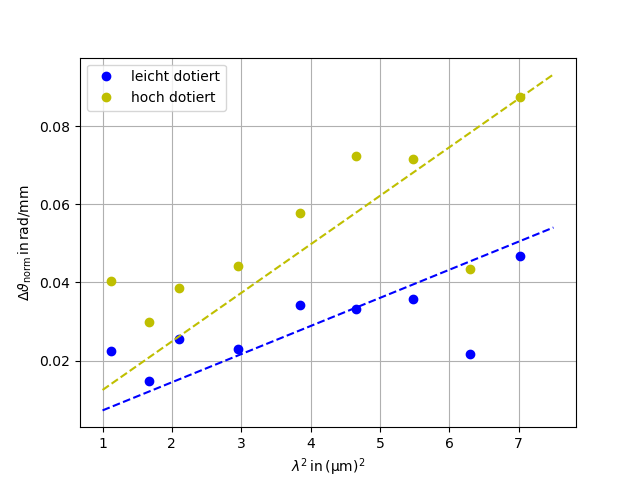
\includegraphics[scale=0.7]{fig/deltaTheta.png}
  \caption{Grafische Darstellung der Messdaten aus den Tabellen \ref{tab:tief} und \ref{tab:hoch}.}
  \label{abb:delta}
\end{figure}
